% Template for Cogsci submission with R Markdown

% Stuff changed from original Markdown PLOS Template
\documentclass[10pt, letterpaper]{article}

\usepackage{cogsci}
\usepackage{pslatex}
\usepackage{float}
\usepackage{caption}

% amsmath package, useful for mathematical formulas
\usepackage{amsmath}

% amssymb package, useful for mathematical symbols
\usepackage{amssymb}

% hyperref package, useful for hyperlinks
\usepackage{hyperref}

% graphicx package, useful for including eps and pdf graphics
% include graphics with the command \includegraphics
\usepackage{graphicx}

% Sweave(-like)
\usepackage{fancyvrb}
\DefineVerbatimEnvironment{Sinput}{Verbatim}{fontshape=sl}
\DefineVerbatimEnvironment{Soutput}{Verbatim}{}
\DefineVerbatimEnvironment{Scode}{Verbatim}{fontshape=sl}
\newenvironment{Schunk}{}{}
\DefineVerbatimEnvironment{Code}{Verbatim}{}
\DefineVerbatimEnvironment{CodeInput}{Verbatim}{fontshape=sl}
\DefineVerbatimEnvironment{CodeOutput}{Verbatim}{}
\newenvironment{CodeChunk}{}{}

% cite package, to clean up citations in the main text. Do not remove.
\usepackage{cite}

\usepackage{color}

% Use doublespacing - comment out for single spacing
%\usepackage{setspace}
%\doublespacing


% % Text layout
% \topmargin 0.0cm
% \oddsidemargin 0.5cm
% \evensidemargin 0.5cm
% \textwidth 16cm
% \textheight 21cm

\title{Exploring a Causal Link between Language and Cultural Biases}


\author{{\large \bf Molly Lewis} \\ \texttt{mollyllewis@gmail.com} \\ Department of Psychology  \\ University of Wisconsin-Madison \And {\large \bf Gary Lupyan} \\ \texttt{lupyan@wisc.edu} \\ Department of Psychology  \\ University of Wisconsin-Madison}

\begin{document}

\maketitle

\begin{abstract}
The abstract.

\textbf{Keywords:}
IAT, cultural biases, gender, linguistic relativity.
\end{abstract}

\section{Introduction}\label{introduction}

\section{Study 1: Cross-cultural gender bias in implicit
behavior}\label{study-1-cross-cultural-gender-bias-in-implicit-behavior}

We quantified the degree of gender bias in a culture using data from the
Implicit Association Task (IAT; Greenwald, McGhee, \& Schwartz, 1998).
The IAT measures the strength of respondents' associations between two
pairs of concepts (e.g., male-career/female-family
vs.~male-family/female-career). The underlying assumption of the measure
is that concepts that are represented as more similar to each other
should be easier to pair together in a behavioral task, compared to two
concepts that are relatively dissimilar. Concepts are paired in the task
by assigning them to the same response keys in a 2AFC categorization
task. In the critical blocks of the task, concepts are assigned to keys
in a way that is either bias-congruent (i.e.~Key A = male/career; Key B
= female/family) or bias-incongruent (i.e.~Key A = male/family; Key B =
female/career). Participants are then presented with a word related to
one of the four concepts and asked to classify it as quickly as possible
by responding with one of the two keys. Slower reaction times in the
bias-incongruent blocks relative to the bias-congruent blocks are
interpretted as indicating an implicit association between the
corresponding concepts (i.e.~a bias to associate male with career, and
female with family).

\subsection{Method}\label{method}

We analyzed an exisiting dataset of IAT scores collected online from a
large, culturally diverse sample (Project Implicit:
\url{https://implicit.harvard.edu/implicit/}; Nosek, Banaji, \&
Greenwald,
2002)\footnote{All analysis code can be found in an online repository: https://github.com/mllewis/IATLANG}.
Our analysis included all gender-career IAT scores collected from
respondents between 2005 and 2016 who had complete data and were located
in countries with more than 400 total respondents (\emph{N} = 773,205).
We further restricted our sample based on participants' reaction times
and errors using the same criteria described in Nosek, Banjai, and
Greenwald (2002, pg. 104). Our final sample included 664,359
participants from 49 countries, with a median of 1,123 participants per
country.

Several measures have been used in the literature to describe the
difference in reaction time between bias congruent and incongruent
blocks. Here, we use the best performing measure, D-score, which
quantifies the difference between critical blocks for each participant
while controling for individual differences in response time (Greenwald,
Nosek, \& Banaji, 2003). For each country, we calculated an effect size
as the mean D-score divided by its standard deviation (Cohen's
\emph{d}), with larger values indicate greater bias.

In addition to the implicit measure, we also analyzed an explicit
measure of gender bias. After completing the IAT, participants were
asked, ``How strongly do you associate the following with males and
females?'' for both the words ``career'' and ``family.'' Participants
indicated their response on a Likert scale ranging from female (1) to
male (7). We calculated an explicit gender bias score for each
participant as the career response minus the family response, such that
greater values indicated more gender bias.

Finally, we also examined an independent measure of gender parity,
called the Women's Peace and Security Index (WPS, 2017), which measures
inclusion, justice, and security of women by country, with larger values
indicating more gender equality. We predicted this measure would be
correlated with measures of implicit and explicit gender bias.

\subsection{Results}\label{results}

\begin{CodeChunk}
\begin{figure}[t]

{\centering 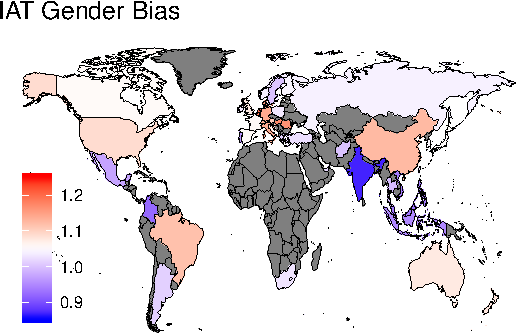
\includegraphics{figs/map-1} 

}

\caption[IAT gender bias effect size for 49 countries with available data]{IAT gender bias effect size for 49 countries with available data. All countries show a gender bias, with red indicating above average and blue indicating below average bias.}\label{fig:map}
\end{figure}
\end{CodeChunk}

Broadly, we replicate previous findings in the literature on the
gender-career IAT (Nosek et al., 2002). First, participants in all
countries showed a bias to associate men with career and females with
family. Figure 1 shows the magnitude of the IAT gender bias (effect
size) across all 49 countries (\emph{M} = 0.37; \emph{SD} = 0.03).
Second, implicit and explicit bias measures were correlated both at the
level of individual participants (\emph{r} = 0.15; \emph{p} \textless{}
.00001) and at the level of countries (\emph{r} = 0.32; \emph{p} =
0.02). Third, consistent with previous findings (Nosek et al., 2002),
the magnitude of the implicit bias is larger for female participants
compared to males (\emph{t} = 97.23; \emph{p} \textless{} .00001).

\begin{CodeChunk}
\begin{figure}[t]

{\centering 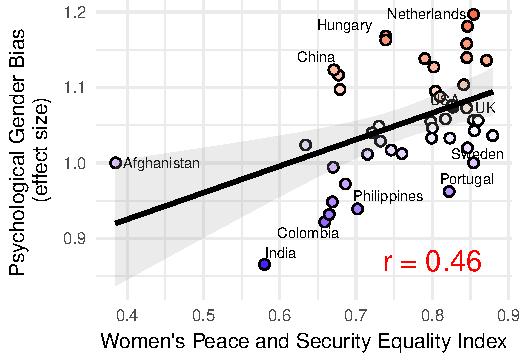
\includegraphics{figs/WPS_plot-1} 

}

\caption[Magnitude of thie implicit gender bias (measured by the IAT) predicted by an indepedent measure of gender equality, Women's Peace and Security Index (WPS)]{Magnitude of thie implicit gender bias (measured by the IAT) predicted by an indepedent measure of gender equality, Women's Peace and Security Index (WPS).  Each point corresponds to a country. Contra our prediction, we find that countries with greater gender equality have larger implicit bias.}\label{fig:WPS_plot}
\end{figure}
\end{CodeChunk}

We next asked whether our independent measure of gender equality, WPS,
predicted variability in implicit and explicit gender bias by country.
WPS was strongly correlated with implicit bias (\emph{r} = 0.46;
\emph{p} = \textless{}.01; Fig.~X), but not explicit bias (\emph{r} =
-0.01; \emph{p} = 0.96). However, we find that the implicit bias effect
is in the opposite of the predicted direction: Countries with higher
gender equality have larger implicit bias.

\subsection{Discussion}\label{discussion}

\section{Study 2: Cross-cultural gender bias in
language}\label{study-2-cross-cultural-gender-bias-in-language}

In Study 2, we ask whether participants' implicit and explicit gender
biases are correlated with biases found in the semantics of
participants' native languages. To model semantics, we turn to a
recently developed machine-learning method for deriving lexical
semantics from text: auto-encoding neural network models. The underlying
assumption of these models is that the meaning of a word can be
described by the words it tends to co-occur with -- an approach known as
distributional semantics (Firth, 1957). Under this approach, a word like
``dog'' is represented more semantically similar to ``hound'' than
``banana'' because it co-occurs with words more in common with ``hound''
than ``banana'' in a large corpus of text.

Recent developments in machine learning allow the idea of distributional
semantics to be implentented in a way that both takes into account many
features of local language structure while remaining computationally
tractable. The best known of these word embedding models is
\emph{word2vec} (Mikolov, Chen, Corrado, \& Dean, 2013). The model takes
as input a corpus of text and outputs a vector for each word
corressponding to its semantics. From these vectors, we can derive a
measure of the semantic similarity between two words by taking the
distance between their vectors (using cosine distance, for example).
Similarity measures estimated from these models have been shown to be
highly correlated with human judgements of word similarity (e.g., Hill,
Reichart, \& Korhonen, 2015).

In addition to quantifying word similarity, models like word2vec have
been used to measure the presence of social biases in the semantics of
English in a way that is highly analogus to the behvioral IAT (Caliskan,
Bryson, \& Narayanan, 2017; henceforth \emph{CBN}). This is done by
measuring the distance in vector space between the same sets of words
that are presented to participants in the IAT task. CBN demonstrate that
these distance measures are highly correlated with reaction times in the
behavioral IAT task, suggesting that the biases measured by the IAT are
also found in the lexical semantics of natural language.

In Study 2, we use the method described by CBN to measure the biases in
the semantics of the natural languages spoken in the countries of
participants in Study 1. While CBN only analyzed biases for models
trained on English, we extend their method to compare biases across a
wide number of languages. To do this, we take advantage of a set of
models that have been pre-trained on a corpus of Wikipedia text in a
large number of languages (Bojanowski, Grave, Joulin, \& Mikolov, 2016).
In Study 2a, we replicate the CBN findings with the Wikipedia corpus; In
Study 2b, we show that the implicit gender biases reported in Study 1
for individual countries are correlated with the biases found in the
semantics of the natural language spoken by those participants.

\subsection{Study 2a: Replication of Caliskan, et
al.~(2017)}\label{study-2a-replication-of-caliskan-et-al.2017}

\subsubsection{Method}\label{method-1}

We use a word embedding model that has been pre-trained model on the
corpus of English Wikipedia using the fastText algorithm (Bojanowski et
al.,
2016)\footnote{Available here: https://github.com/facebookresearch/fastText/}.
The model contains 2,519,370 words with each word reprsented by a 300
dimension vector.

Using the Wikpedia fastText model, we calculate an effect size for each
of the 10 biases reported in CBN which correspond to behavioral IAT
results existing in the literature: flowers/insects/pleasant/unpleasant,
instruments/weapons/pleasant/unpleasant,
European-American/Afro-American/pleasant/unpleasant\footnote{CBN test three versions of this bias.},
males/females/career/family, math/arts/male/female,
science/arts/male/female, mental disease/physical
disease/permanent/temporary, and young/old/pleasant/unpleasant (labeled
as WEAT 1-10 in CBN). We calculate the bias using the same effect size
metric described in CBN, a standardized difference score of the relative
similarity of the target words to the target attributes (i.e.~relative
similarity of male to career vs.~relative similarity of female to
career). This measure is analagous the behavioral effect size measure in
Study 1 and, like for the behavioral effect size, larger values indicate
larger bias.

\subsubsection{Results}\label{results-1}

\begin{CodeChunk}
\begin{figure}[t]

{\centering 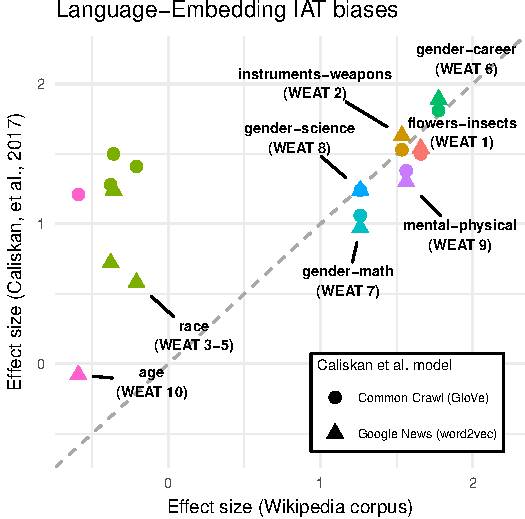
\includegraphics{figs/WEAT_plot-1} 

}

\caption[Effect sizes for the 10 IAT biases types (WEAT 1-10) reported in Caliskan et al]{Effect sizes for the 10 IAT biases types (WEAT 1-10) reported in Caliskan et al. (2017; CBN). The effect sizes reported in CBN are plotted against  effect sizes from the Wikipedia corpus.  Point color corresponds to  bias type, and point shape corresponds to the two CBN models trained on different corpora and with different algorithms.}\label{fig:WEAT_plot}
\end{figure}
\end{CodeChunk}

Figure 2 shows the effect size measures derived from the Wikipedia
corpus plotted against effect size esimtates reported by CBN from two
different models (trained on the Common Crawl and Google News corpora).
With the exception of biases related to race and age, effect sizes from
the Wikipedia corpus are comparable to those reported by CBN. In
particular, for the gender-career IAT -- the bias relevant to our
current purposes -- we estimate the effect size to be 1.78, while CBN
estimates it to be 1.81 (Common Crawl) and 1.89 (Google News).

\subsection{Study 2b: Predicting implicit bias with language
IAT}\label{study-2b-predicting-implicit-bias-with-language-iat}

With our corpus validated, we next turn toward examining the
relationship between psychological and linguistic gender biases. In
Study 2b, we estimate the magnitude of the gender-career bias in each of
the languages spoken in the countries described in Study 1 and compare
it with estimates of behavioral gender bias from Study 1. If language
causally influences psyschological gender bias, we predict these two
measures should be positively correlated.

\subsubsection{Method}\label{method-2}

\begin{CodeChunk}
\begin{figure}[t]

{\centering 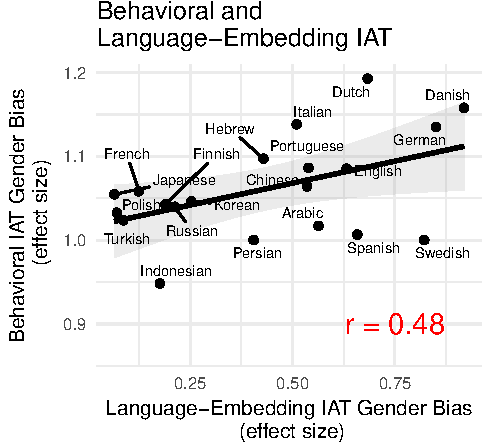
\includegraphics{figs/behavior_vs_language_plot-1} 

}

\caption[Gender bias effect size for each language from the behavioral IAT task (averaging acrouss countries]{Gender bias effect size for each language from the behavioral IAT task (averaging acrouss countries; Study 1) versus gender bias effect size estimated from embedding models trained on each language.}\label{fig:behavior_vs_language_plot}
\end{figure}
\end{CodeChunk}

For each country included in Study 1, we identifed the most frequently
spoken language in those countries using the CIA factbook (Central
Intelligence Agency, 2017). This included a total of 32 unique
languages. For a sample of 20 of these languages (see Fig.~3), we had
native speakers translate the set of 32 words from the gender-career
IAT, with a slight modification
\footnote{The language sample was determined by accessibility to native speakers, but included languages from a variety of language families.}.
The original gender-career IAT task (Nosek et al., 2002) used proper
names to cue the male and female categories (e.g. ``John,'' ``Amy'').
Because there are not direct translation equivalents of proper names
across languages, we instead used a set of generic gendered words which
had been previously used for a different version of the gender IAT
(e.g., ``male,'' ``man,'' ``female,'' ``woman;'' Nosek et al., 2002).

We used these translations to calculate an effect size from the models
trained on Wikipedia in each language, using the same methood as in
Study 2a. We then compared the effect size of the linguistic gender bias
to the behavioral gender bias across, averaging across countries that
spoke the same language (weighting by sample size).

\subsubsection{Results}\label{results-2}

Implicit IAT gender bias effect sizes were positively correlated with
effect sizes of gender bias estimated from the native language embedding
model (\emph{r} = 0.48; \emph{p} = 0.03; Fig.~3), suggesting that
countries that have more gender bias encoded in their language also have
a larger psychological gender bias. Explicit gender bias was not
reliably correlated with language gender bias (\emph{r} = 0.23; \emph{p}
= 0.32).

\subsection{Discussion}\label{discussion-1}

\section{Study 3: Grammar and Gender
Bias}\label{study-3-grammar-and-gender-bias}

Study 2 suggests that psychological gender bias and linguistic gender
bias are correlated, consistent with the idea that language may play a
causal factor in shape gender bias in behavior. Nevertheless, Study 2 is
also consistent with a second hypothesis in which the causal influence
goes the opposition direction: Psychological gender bias leads to a
gender bias becoming encoded in the language. In Study 3, we test the
causal hypothesis more directly by examining whether there is a
relationship between psychological gender bias and language along a
linguistic dimension that is unlikely to be subject to change -- namely,
grammatical gender. While of course grammars do change, they are less
malleable than the semantics of words, and thus less likely to be
affected by psychological biases. We predict, therefore, that if there
is some causal influence of language on psycholgical biases languages
that encode gender grammatically will tend to have larger psychological
gender biases.

\subsection{Method}\label{method-3}

\subsection{Results}\label{results-3}

\subsection{Discussion}\label{discussion-2}

\section{Study 4: exploring bias more
directly}\label{study-4-exploring-bias-more-directly}

\section{to do}\label{to-do}

does anything predict gender inqequality in study 1 (that paper i saw)
explain language != culture thing a bunch more words for google
translate break down men vs women (?)

\section{Conclusion}\label{conclusion}

\section{References}\label{references}

\setlength{\parindent}{-0.1in} \setlength{\leftskip}{0.125in} \noindent

\hypertarget{refs}{}
\hypertarget{ref-bojanowski2016enriching}{}
Bojanowski, P., Grave, E., Joulin, A., \& Mikolov, T. (2016). Enriching
word vectors with subword information. \emph{arXiv Preprint
arXiv:1607.04606}.

\hypertarget{ref-caliskan2017semantics}{}
Caliskan, A., Bryson, J. J., \& Narayanan, A. (2017). Semantics derived
automatically from language corpora contain human-like biases.
\emph{Science}, \emph{356}(6334), 183--186.

\hypertarget{ref-ciafactbook}{}
Central Intelligence Agency. (2017). The World Factbook. Retrieved from
\url{ttps://www.cia.gov/library/publications/the-world-factbook/index.html}

\hypertarget{ref-firth1957synopsis}{}
Firth, J. (1957). A synopsis of linguistic theory 1930-1955 in studies
in linguistic analysis, philological society. Oxford. reprinted in
Palmer, F.,(ed. 1968), Selected Papers of JR Firth, Longman, Harlow.

\hypertarget{ref-greenwald1998measuring}{}
Greenwald, A. G., McGhee, D. E., \& Schwartz, J. L. (1998). Measuring
individual differences in implicit cognition: The implicit association
test. \emph{Journal of Personality and Social Psychology}, \emph{74}(6),
1464.

\hypertarget{ref-greenwald2003understanding}{}
Greenwald, A. G., Nosek, B. A., \& Banaji, M. R. (2003). Understanding
and using the implicit association test: I. an improved scoring
algorithm. \emph{Journal of Personality and Social Psychology},
\emph{85}(2), 197.

\hypertarget{ref-hill2015simlex}{}
Hill, F., Reichart, R., \& Korhonen, A. (2015). Simlex-999: Evaluating
semantic models with (genuine) similarity estimation.
\emph{Computational Linguistics}, \emph{41}(4), 665--695.

\hypertarget{ref-mikolov2013efficient}{}
Mikolov, T., Chen, K., Corrado, G., \& Dean, J. (2013). Efficient
estimation of word representations in vector space. \emph{arXiv Preprint
arXiv:1301.3781}.

\hypertarget{ref-nosek2002harvesting}{}
Nosek, B. A., Banaji, M. R., \& Greenwald, A. G. (2002). Harvesting
implicit group attitudes and beliefs from a demonstration web site.
\emph{Group Dynamics: Theory, Research, and Practice}, \emph{6}(1), 101.

\hypertarget{ref-wps}{}
Women's Peace and Security Index. (2017). Retrieved from
\url{https://giwps.georgetown.edu/}

\end{document}
